\begin{figure}[h]
    \centering
    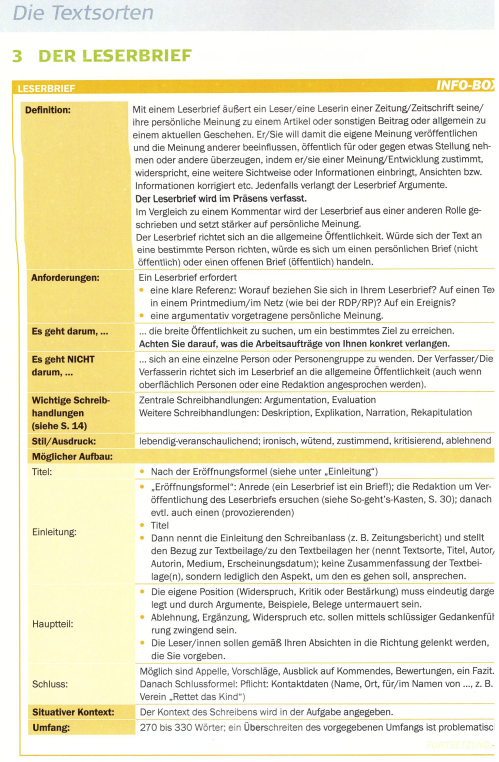
\includegraphics[scale=0.8]{./pics/Screenshot from 2023-02-06 12-28-25.png}
    \caption{Leserbrief: Definition + Aufbau}
    \label{fig:impl:Leserbrief1}
\end{figure}

\begin{figure}[h]
    \centering
    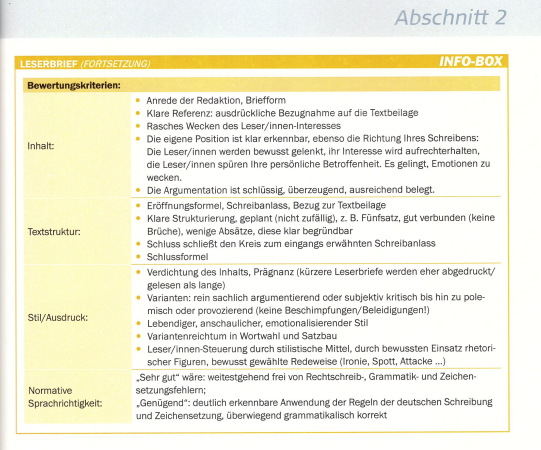
\includegraphics[scale=0.8]{./pics/Screenshot from 2023-02-06 12-28-55.png}
    \caption{Leserbrief: Verfassen}
    \label{fig:impl:Leserbrief2}
\end{figure}
\begin{figure}[h]
    \centering
    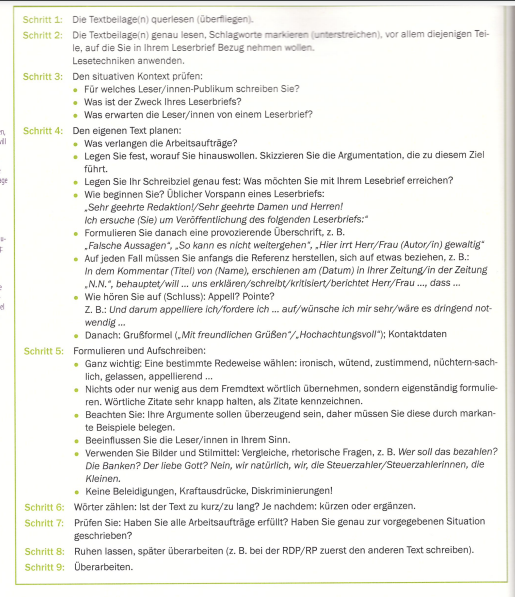
\includegraphics[scale=0.8]{./pics/Screenshot from 2023-02-06 12-29-05.png}
    \caption{Leserbrief: Fortsetzung}
    \label{fig:impl:Leserbrief3}
\end{figure}



\section{Mustertext}

Sehr geehrte Redaktion! 

Ich ersuche Sie um die Veröffentlichung des folgenden Leserbriefs: 
\subsubsection{Sexy und sexistisch  Muss das sein? }

Als ich die Kolumne „Sexy und sexistisch“ von Niki Glattauer, erschienen am 18. März 2013 in der Tageszeitung Kurier las, schoss mir sofort eine Frage durch den Kopf: Muss sowas denn wirklich sein?  

Herr Glattauer berichtet von einem sexistischen Werbeplakat der Wiener Linien. Darauf ist ein Mann zusehen, der seinen Allerwertesten direkt auf zwei elegant gekleidete Frauen, welche sich gerade unterhalten, gerichtet hat. Dabei sagt die eine Frau kichernd zu der anderen: Ich sagte doch, du sollst mehr Bus fahren. Niki Glattauer dreht daraufhin die Situation um und erläutert, dass ein Plakat mit zwei Männern in Anzug, die über den Hintern einer Frau feixen, ohne Berechtigung, als sexistisch oder unpassend abgestempelt werden würde. Herr Glattauers betont, dass ein klarer Unterschied zwischen sexy und sexistisch besteht. Denn das einzige, das vom Werbeplakat betont wird, ist der Hintern des Mannes. Kein Mann muss sich dadurch belästigt fühlen.  

Man kann das Ganze jedoch auch anders sehen. Die Ansicht, die man mit der Thematik verbindet, ist immer abhängig von den Gedanken oder Erinnerungen der Person. Manche Menschen ärgern sich über die Werbung und meinen sie sei unpassend und wieder andere lachen darüber und denken sich nichts weiter dabei.  

Da Sexismus leider auch heute noch immer eine sehr große Rolle in unserer Gemeinschaft spielt, muss man doch nicht mehr Wirbel über das Thema verbreiten, als ohnehin schon besteht. Ich gebe Herrn Glattauer mit der Überlegung, dass sexy nicht gleich sexistisch meint, zwar recht, jedoch kann man doch auf diese Anspielungen bei einer Werbung verzichten. Viele Leute fühlen sich dadurch persönlich angegriffen, beschämt oder gar verletzt und wohin sollen diese Gefühle bei der Debatte des Sexismus führen?  

\section{Eigener Text}
\subsection{Angabe}
\subsubsection{Körperbilder }

Verfassen Sie einen Leserbrief. 

Situation: Im Rahmen eines Projekts Ihrer Klasse bzw. Ihres Kurses zum Thema Körperbilder verfassen Sie einen Leserbrief, der auf der Projektwebsite veröffentlicht wird und für den Sie auch einen passenden Titel formulieren. 

Lesen Sie den Bericht Beauty-Apps: Die Macht der Influencer von Selina Thaler aus der OnlineAusgabe der Tageszeitung Der Standard vom 26. Jänner 2019 (Textbeilage 1). Verfassen Sie nun den Kommentar und bearbeiten Sie dabei die folgenden Arbeitsaufträge: 

\begin{compactitem}
    \item Geben Sie wieder, wodurch Selbstwahrnehmung und Körperbild laut Textbeilage beeinflusst werden.  
    \item Nehmen Sie dazu Stellung. 
    \item Bewerten Sie im Text genannte Maßnahmen und Initiativen, um der dargestellten Problematik entgegenzuwirken. 
\end{compactitem}

\subsubsection{Beauty-Apps: Die Macht der Influencer}

Kaum jemand beeinflusst das aktuelle Schönheitsideal so sehr wie diese Influencer – und das meist mithilfe
von Retusche-Apps. Das kann zu Selbstwahrnehmungsstörungen führen, warnen Experten


Ein Klick, und die Falten sind
geglättet, die Pickel verschwunden. Ein Wisch, und die Lippen
sind voller, die Nase kleiner, die
Augen strahlender.
Nie war es so einfach, sein Gesicht
vermeintlich zu verschönern oder
kleine Makel verschwinden zu
lassen. In die Kameras der neuen
Smartphone-Generation sind
Selfie-Filter bereits fix einprogrammiert, dazu boomen kostenpflichtige Retusche-Apps. [...]
Dabei geht es nicht nur darum,
den Teint makelloser zu filtern, die
Zähne aufzuhellen oder dunkle
Augenringe verschwinden zu lassen. Man kann auch das Kinn
zuspitzen, schlaffe Augenlider
straffen, Wangenknochen anheben oder die Hüfte verschmälern – es ist quasi die SchönheitsOP per Klick, schmerzfrei und
kostengünstig.
Klingt absurd? Mitnichten. Die
Nachfrage bestimmt den Markt
[...]. Turbo hinter dem Filterboom ist die Fotoplattform Instagram mit ihrer weltweit über
einen Milliarde Nutzer, die im
Schnitt 80  Millionen Fotos pro
Tag teilen. Umfragen zeigen, dass
die Mehrheit der User die Fotos
erst bearbeitet, ehe sie sie postet.
Gefilterte Wahrnehmung
Instagram, Snapchat und viele
andere Anwendungen haben ihre
Benutzer darin geschult, jene
Werkzeuge zur Bildbearbeitung
zu benutzen, die in Vor-SocialMedia-Zeiten ausschließlich Bildredakteuren von Fashion-Magazinen oder Werbegrafikern vorbehalten waren. Heute steht der
Da-lässt-sich-noch-was-machenJungbrunnen jedem offen.
Das, so meinen Experten, kann
deutlichen Einfluss auf die Selbstwahrnehmung und das Körperbild haben. Denn durch soziale
Medien ergebe sich eine neue
Dynamik, weil man dort mit so
vielen Bildern wie noch nie zuvor
konfrontiert werde, sagt der Psychologe Helmut Leder, der sich
an der Universität Wien mit
der Wahrnehmung von Ästhetik beschäftigt. „Unser Wahrnehmungssystem kann nicht
zwischen unbearbeiteten und
retuschierten Fotos unterscheiden und verarbeitet jedes Bild“,
sagt Leder. „Dadurch wird unser
Prototyp einer schönen Person zunehmend mit Merkmalen
gefüttert, die nichts mit der Wirklichkeit zu tun haben.“
Auf diese Weise prägt Instagram,
wie Körper in der Gesellschaft
dargestellt und wahrgenommen
werden. Es entsteht eine perfekte, digitale Parallelgesellschaft
und eine Realität voll wandelnder
Mogelpackungen. [...]
Denn erstens werde vermittelt,
dass nur das Aussehen zählt und
nicht die Persönlichkeit, erklärt
[...] die Medienwissenschafterin Katrin Döveling, die Studien
zu dem Thema veröffentlicht hat.
„Zweitens erzeugt es Druck, dass
man nicht genügt, nicht schön
oder dünn genug ist. Dabei ist
niemand perfekt.“ Dieser Druck
und das ständige Bewertetwerden
führen dazu, dass „quasi jeder
seine Fotos bearbeitet“.
Bearbeitungswahn
[...] Der Bearbeitungswahn ist
aber nur die kleinste Auswirkung. „Haben sich Menschen
bereits einen solchen unnatürlichen Prototyp gebildet, werden

lle möglichen Störungen des
Selbst- und Körperbildes wie
etwa Anorexie oder Depressionen
wahrscheinlicher“, erklärt der
Psychologe Leder. Auch Neid
und Minderwertigkeitsgefühle
entstünden. Es gibt sogar einen
Begriff für die durch soziale
Medien ausgelöste Unzufriedenheit mit dem eigenen Körper:
Snapchat-Dismorphia.
Für die meisten sind solche Apps
eine harmlose Spielerei. Doch
Experten vermuten, dass immer
mehr offline so aussehen wollen
wie ihr Online-Alter-Ego. Das
legt auch eine 2017 vom amerikanischen Verband für Plastische
Chirurgie weltweit durchgeführte
Befragung von Schönheitschirurgen nahe: Mehr als die
Hälfte der Befragten gab an, dass
Patienten Eingriffe nur vornehmen lassen wollten, um auf Selfies
besser auszusehen. Diesen Trend
kann der plastische Chirurg Thomas Aigner für Österreich nicht
ausmachen: „Ich bezweifle, dass
sich jemand deshalb operieren
lässt. Höchstens bei kleineren
Eingriffen wie Botox, Hyaluron
oder Fadenlifting kann ich mir
das vorstellen – und das auch nur
bei wenigen Personen.“
Bei der Österreichischen Gesellschaft für Plastische Chirurgie
beobachtet man, dass manche
Patienten mittlerweile retuschierte Selfies zur Behandlung
mitnehmen, früher waren es Fotos
aus Hochglanzmagazinen. Das
habe er in seiner Ordination noch
nicht erlebt, sagt Aigner. Und er
wäre vorsichtig, danach zu operieren: „Auf dem Bild entscheidet
nicht nur die schmale Nase, sondern auch die Gesichtszüge, die
Hautfarbe, die Porengröße. Zwischen Bild und Wirklichkeit ist
immer ein Gap.“
Junge besonders betroffen
Besonders junge Frauen seien von
der übermäßigen Retusche und
den daraus resultierenden psychischen Folgen betroffen, da sie
noch nicht so in ihrem Selbstwert
gefestigt seien, sagt die Medienwissenschafterin Döveling. Denn
die scheinbar perfekten Influencerinnen sind für diese Zielgruppe
oft Vorbilder. Die Kognitionsforscherin Dayana Hristova untersucht in ihrer Dissertation […]
an der Uni Wien, wie sich digitale
Selbstoptimierung auf Jugendliche auswirkt. Wer Selfies postet,
bearbeitet sie auch. „Je mehr man
von sich zeigt, desto mehr hat man
das Bedürfnis, sich zu optimieren.“ Dennoch relativiert sie: „Die
Jungen haben eine realistische
Einschätzung und wissen, dass sie
nicht alles für wahr nehmen können, was sie auf Instagram sehen.“
Aufklärung sei trotzdem wichtig.
Zumal man davon ausgehen muss,
dass sich nicht jeder der Manipulation der Bilder bewusst ist.
In Österreich wollte die ehemalige Frauenministerin Gabriele Heinisch-Hosek (SPÖ) 2015
eine Kennzeichnungspflicht für
retuschierte Bilder durchsetzen. Doch daraus wurde nichts.
In Frankreich hingegen muss die
Bearbeitung von Fotos in Magazinen oder Werbung seit rund
einem Jahr ausgewiesen werden.
Bislang kaum thematisiert ist die
Kennzeichnung von Bildretusche
in sozialen Medien. Für den Psychologen Helmut Leder greifen
all diese Regelungen viel zu kurz:
„Auch wenn es für die künstlerische Freiheit heikel ist, würde es
helfen, wenn Länder solche Manipulationen grundsätzlich verböten oder zumindest reduzierten.“
Denn der Betrachter eines Fotos
nimmt die Kennzeichnung zwar
wahr, doch das Hirn teilt nicht in
manipulierte und unverfälschte
Fotos, sondern verarbeitet alle als
Realität.
Doch es gibt bereits eine Gegenbewegung: Die Bildagentur Getty,
die Modekette Asos und die Kosmetikmarke Dove zeigen Models
unretuschiert  – mit Fettpölstern
und Cellulite. Sie sollen vermitteln, dass sich jeder in seinem
Körper wohl und attraktiv fühlen darf. So wie die Anhänger
der Bodypositivity-Bewegung
auf Instagram ungeschönte Fotos
posten. „Das füttert unseren Prototyp eines schönen Menschen
mit vielfältigeren Körpern, das
ist gut“, sagt Leder. Er rät: Wer
Sorge hat, zu sehr von der Scheinwelt beeinflusst zu werden, solle
sich Leute auf der Straße oder in
der U-Bahn bewusster ansehen.
Sollte auch das nicht helfen, gibt
es Unterstützung  – natürlich per
App: MakeApp schminkt die
Personen auf den Selfies wieder
ab.


Schreiben Sie zwischen 270 und 330 Wörter. Markieren Sie Absätze mittels Leerzeilen.

\subsection{Text}
\subsubsection{Beauty-Apps: Die Macht der Influencer }

Der Artikel von Selina Thaler über die Auswirkungen von Sozial Media und vor allem bearbeitet Bilder auf junge Frauen war einer der informativste Artikel, den ich seit Langem gelesen habe. Und dennoch frage mich, wieso ist das angesprochene Problem in der heutigen, aufgeklärten Zeit immer noch so ein Problem? 

Konkret geht es um die Auswirkungen, welche retuschierte Bilder auf unser Gehirn haben. Welche Folgen dies haben kann und dass es sogar Depressionen und starke Eifersucht auslösen kann. Und das ganz unterbewusst, ohne dass die Nutzer etwas davon mitbekommen. Vor allem die Vorbildfunktion der Influencer spielt hier eine starke Rolle. Viele jugendliche Mädchen, die selbst oft noch kein Selbstwertgefühl haben, wollen oft so perfekt aussehen wie die Menschen auf den Selfies auf Instagram. Snapchat-Dismorphia nennt man diese Unzufriedenheit, die durch die Verbreitung falscher und bearbeiteter Bilder ausgelöst wurden. 

Trotz geplanter Gegenmaßnahmen finde ich es schrecklich, dass durch Apps wie Instagram ein solch falsches Bild von dem menschlichen Körper an junge Menschen geliefert wird. Es ist schlimm, dass sich Mädchen abhungern oder Essstörungen aufbauen, nur um genauso dünn zu sein wie Models im Internet oder im Fernsehen. Doch viele dieser Fotos sind einfach bearbeitet und entsprechen nicht der Realität. Ich finde es gut, dass es schon Versuche gibt, solche Bilder zu markieren oder Models mit „Schönheitsfehler“ zu nehmen. Trotzdem müsste man meiner Meinung schon im Kindesalter die Menschen aufklären und über solche Fallen informieren. Denn trotz jeder Markierung, das Gehirn vergleicht sich trotzdem unterbewusst immer mit anderen. 

Ich rufe Sie, liebe Leser, dazu auf, ihre Söhne und Töchter darüber aufzuklären! Jeder sollte wissen, wie falsch Menschen auf Sozial Media sind, wie viele falsche Sachen viel zu viel Aufmerksamkeit bekommen, und vor allem, dass jeder Körper schön ist. Egal wie er geformt ist, wie viel man wiegt und wie groß die Kurven von jemanden sind. 

302 Wörter 

\newpage


\section{Formulierungshilfen}

Aufbau eines Leserbriefs: 
\begin{compactitem}
    
    \item Anrede: z.B. Name des Redakteurs: Sehr geehrter Herr Schuster! 
    \item Genaue Angabe des Artikels, auf den du dich beziehst: Datum und Überschrift des Artikels, Erscheinungsort 
    \item Schreibabsicht 
\end{compactitem}
So könntest du beginnen: 
\begin{compactitem}
    \item Sie schreiben in Ihrem Artikel (Titel) vom (Datum), der (wo) erschienen ist, dass ….. Dazu möchte ich Ihnen Folgendes mitteilen: … 
    \item Mit Interesse habe ich Ihren Artikel (Titel) vom (Datum) im (Ort) gelesen und frage mich … 
    \item Ihr Beitrag zum Thema … berührt mich sehr. Auch ich habe ähnliche Erfahrungen gemacht. 
    \item In Ihrem Artikel (Titel) vom (Datum) schreiben Sie, dass … 
    \item In seinem Beitrag schreibt Herr Huber, dass … 
    \item Endlich war in Ihrer Zeitung zu lesen, was ich mir schon immer gedacht habe: … 
    \item Ihr Artikel (…) erscheint mir inhaltlich wichtig, schon alleine deshalb, weil 
\end{compactitem}
Im Hauptteil beurteilst du 
\begin{compactitem}
    \item Auch ich habe den Eindruck, dass 
    \item Auch ich habe diese Erfahrung gemacht … 
    \item  Diese Situation kenne ich sehr gut … 
    \item Diese Aussagen entsprechen auch meinen Erfahrungen 
    \item Diese Meinung / Sichtweise kann ich ganz und gar nicht teilen.  
    \item Ich sehe das überhaupt nicht so wie Herr Huber! 
\end{compactitem}
\subsection{Realitätsbezug}
Leserbriefe (Textsorte) findet man oft in Zeitungen oder Zeitschriften, besonders in Print-Medien. Sie dienen als Plattform für die Meinungen und Ansichten der Leser zu aktuellen Themen oder Ereignissen. Leserbriefe können auch in Form von Online-Kommentaren auf Nachrichtenwebsites oder in sozialen Medien veröffentlicht werden. 

\subsection{Erklärung}

Ein Leserbrief ist eine Textsorte, die von einem Leser verfasst wird, um seine Meinung zu einem Thema oder einem Ereignis auszudrücken, das in den Medien behandelt wurde. Leserbriefe werden oft in Zeitungen oder Zeitschriften veröffentlicht und dienen dazu, die Perspektive der Leser zu zeigen und ihre Meinung zu einem bestimmten Thema zu artikulieren.

Leserbriefe sind in der Regel kürzer und informeller als andere Textsorten, wie zum Beispiel Kommentare, und haben einen direkteren Bezug zu einem bestimmten Thema oder Ereignis, das in den Medien behandelt wurde. Sie können auch kontroversielle Themen ansprechen und eine Meinung zu einem Thema darstellen, das für den Autor wichtig ist.
\subsection{Beispiele für verwandte Textsorten}
offener Brief, Posting
\subsection{Abgrenzung}
Der offene Brief richtet sich nicht an ein konkretes Medium (z.B. um
diesem zu widersprechen), sondern an eine breite Öffentlichkeit; dabei
bedient er sich mitunter eines Mediums, ohne auf dessen Berichterstattung Bezug zu nehmen.
\subsection{Umfang} 270– 330 Wörter
\subsection{situativer Kontext} erforderlich
\subsection{Eigene Erfahrung} Eine recht einfache Textsorte, bei der es nur darum geht, seine eigene Meinung anhand des gegebnen Textes freundlich rüber zu bringen. 